\documentclass[11pt]{article}\usepackage[T1]{fontenc}\usepackage[margin=.7in]{geometry}\usepackage{graphicx,booktabs,longtable,amsmath}\setlength{\parindent}{0pt}\begin{document}\section*{No CL versus CL: complete validation comparison}
All replay controllers are displayed even if they fail selection. CL beta 1.0: 7 failed return simulations; all later-case force constraints passed; CL beta 4.0: 4 failed return simulations; force constraints failed in B\_60. No replay candidate qualified under the original selection rule. These results do not establish a CL benefit. DIAGNOSTIC: initial quality did not meet every reference limit in the source run. No winner is selected; all fixed methods are measured, including failures. Current initial quality: 14/15 validation references pass. A lower average over surviving episodes must not hide failed episodes.

Validation only. Seed 42. Failed runs are not assigned an invented final RMSE.
\begin{center}\small\begin{tabular}{lrrrr}\toprule Controller & Completed & Failed & Passed & Mean RMSE$^*$\\\midrule
No CL & 15/15 & 0 & 6/15 & 3.3862\\
CL beta 1 & 8/15 & 7 & 7/15 & 2.2289\\
CL beta 4 & 11/15 & 4 & 7/15 & 5.0231\\
\bottomrule\end{tabular}\end{center}
$^*$Degrees; completed episodes only. Always interpret together with failure counts.
\subsection*{Architecture and training objective}28 inputs, two hidden layers of 64 tanh neurons, and one cable force output. The original implemented objectives are unchanged:\[L_{\mathrm{NoCL}}=\ell_w(D_t)+0.1R(D_t),\quad L_{\mathrm{CL}}=L_{\mathrm{NoCL}}+\beta[\ell_w(M_A)+0.1R(M_A)]\]Here $D_t$ is current-case training data; $M_A$ is the fixed 1,024-example case A buffer; at most 512 are replayed per update. $\ell_w$ is weighted normalized-force mean squared error; $R$ is the original local corrective-response penalty. Beta values are 1, 4 and 16. These are not three independent random seeds.
\clearpage\section*{All Methods Summary}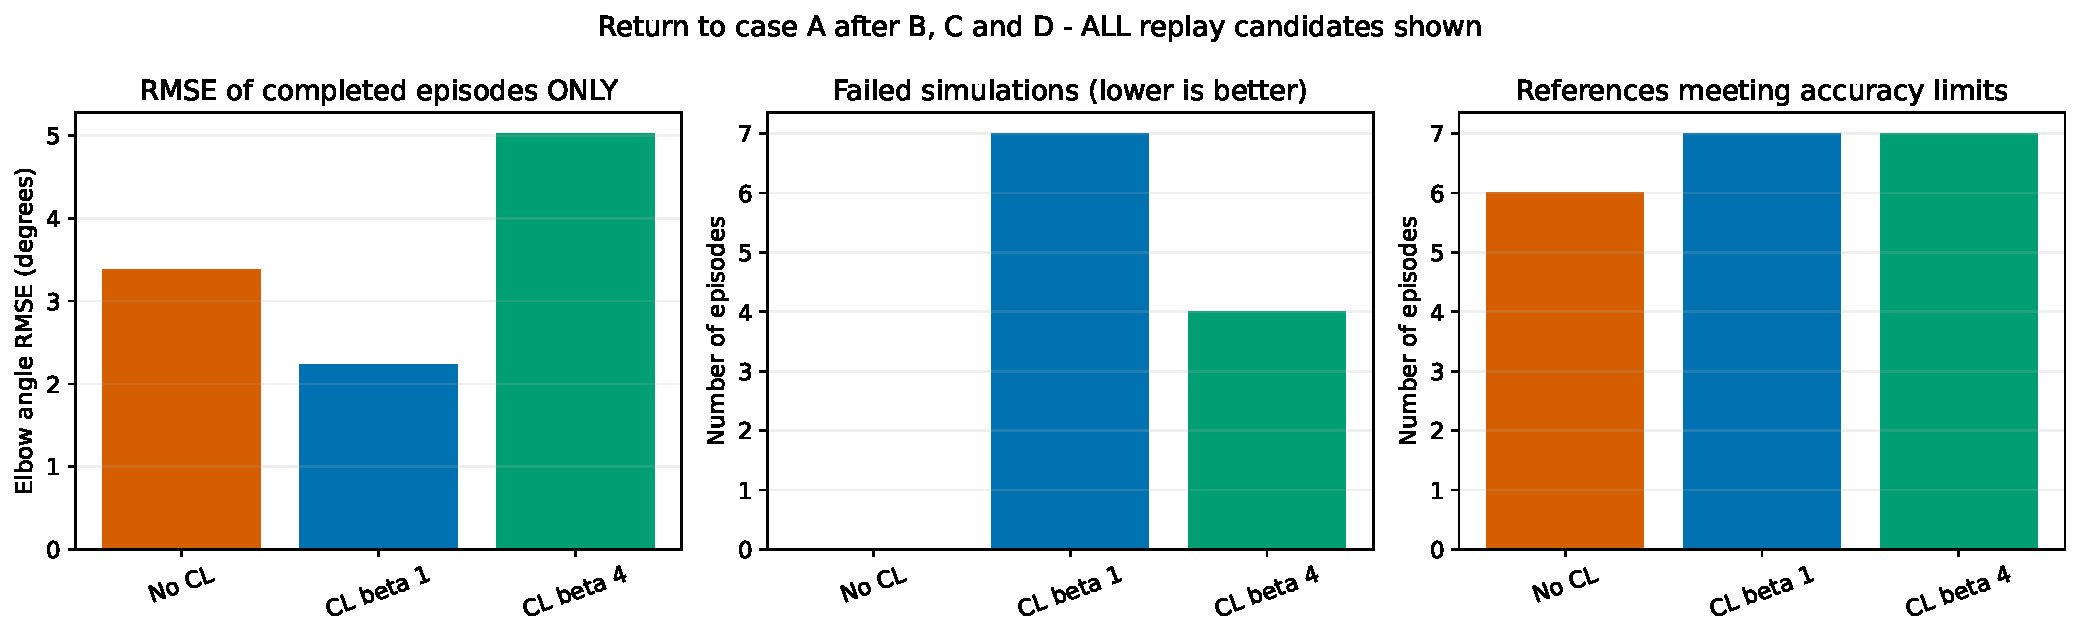
\includegraphics[width=\linewidth,height=.82\textheight,keepaspectratio]{figures/all_methods_summary.pdf}
\clearpage\section*{Every Reference}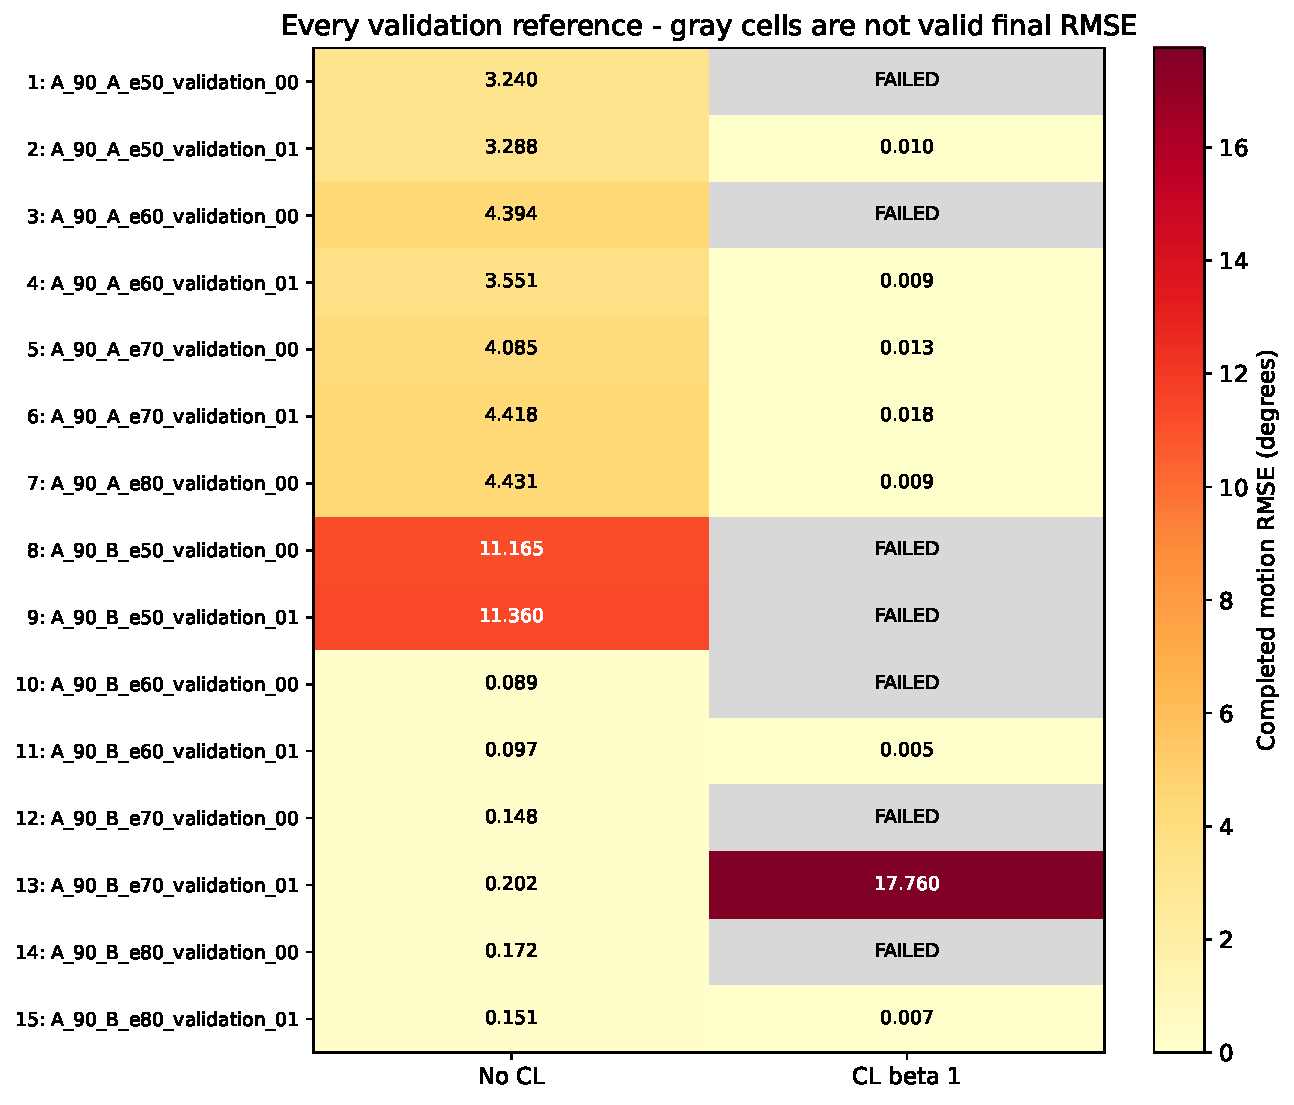
\includegraphics[width=\linewidth,height=.82\textheight,keepaspectratio]{figures/every_reference.pdf}
\clearpage\section*{Learning And Adaptation}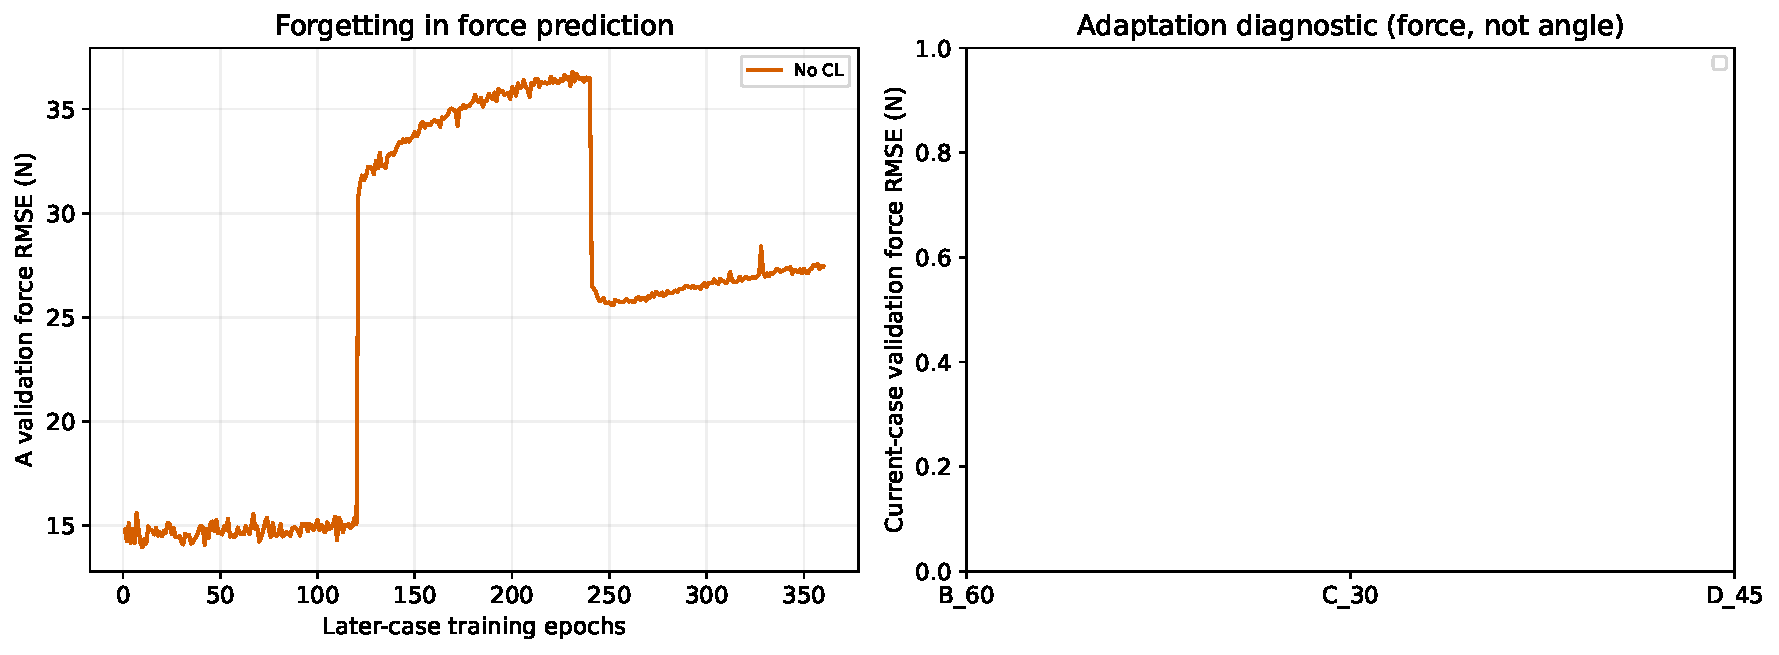
\includegraphics[width=\linewidth,height=.82\textheight,keepaspectratio]{figures/learning_and_adaptation.pdf}
\clearpage\section*{Reference 01}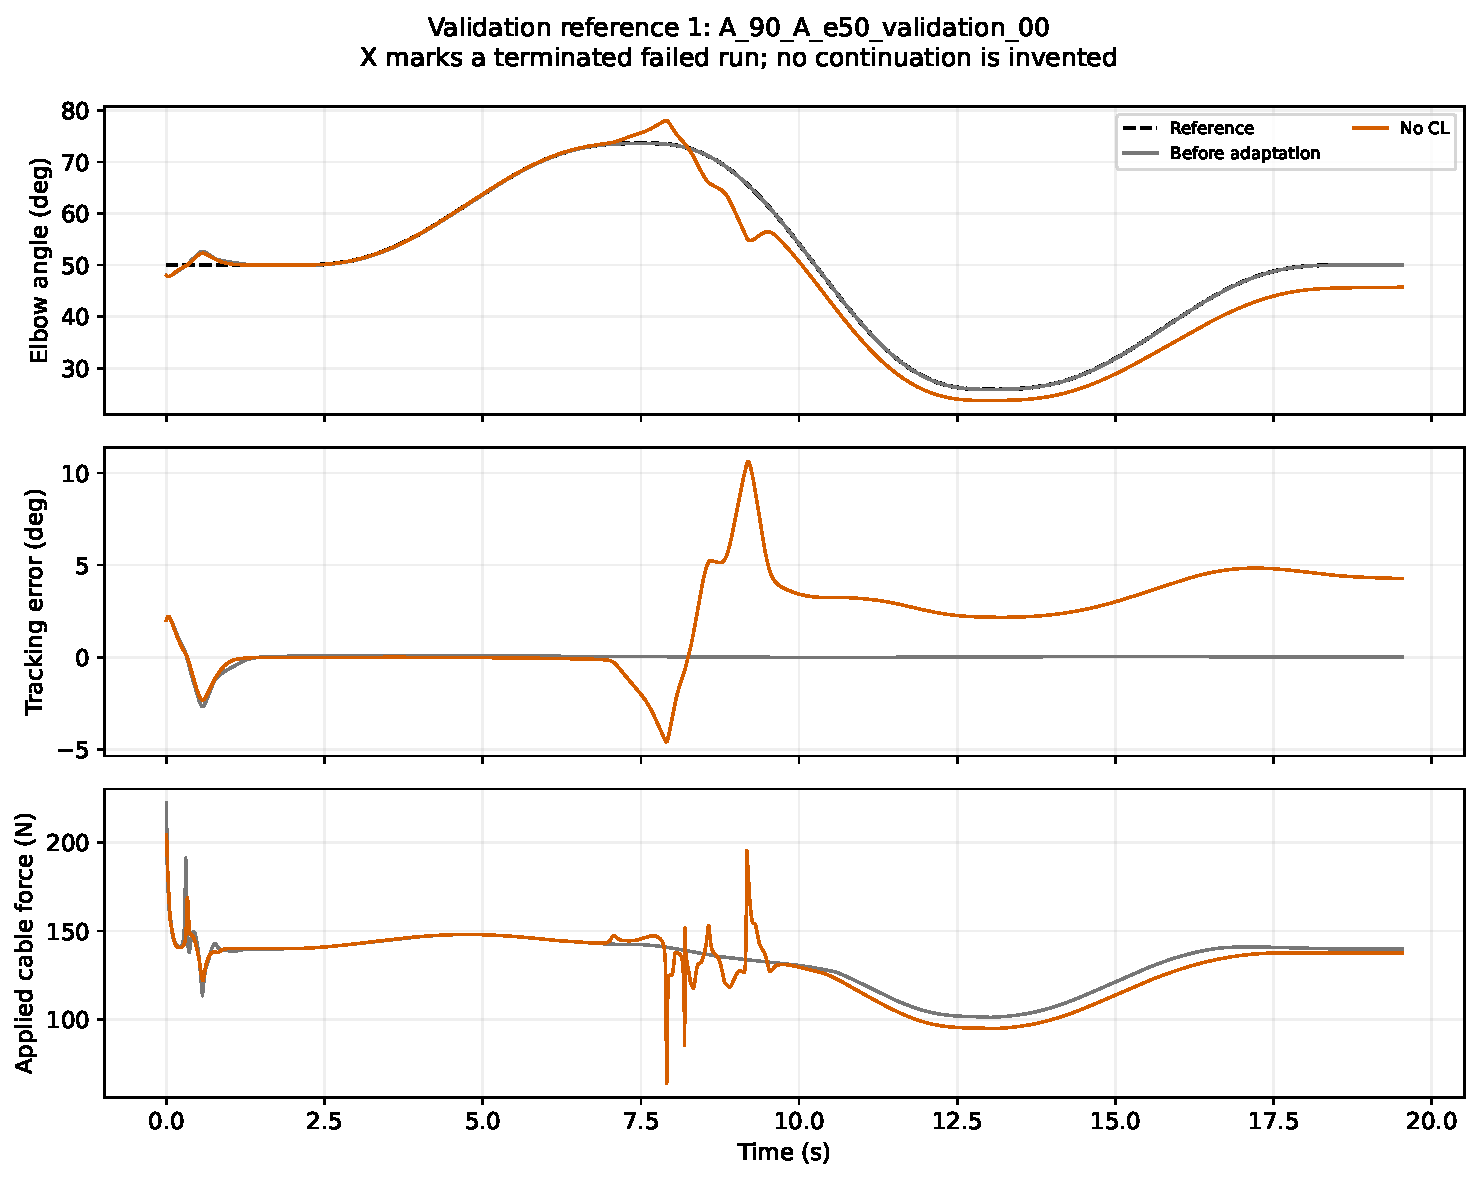
\includegraphics[width=\linewidth,height=.82\textheight,keepaspectratio]{figures/reference_01.pdf}
\clearpage\section*{All reference plots}\small All remaining reference figures are supplied in figures/ for presentation use. Uncomment the include lines in appendix_figures.tex to add them. Original selection and test-lock rules are preserved. No CL superiority is claimed when the measurements do not support it.\end{document}